Shelby Solomon's individual development plan is based on the strengths and weaknesses listed in section~\ref{sec:weaknesses} and will build off of the background~\ref{sec:background}.

\subsection{Technical \& Research Aims}

\begin{description}
	\item[Aim] Differential privacy algorithm development and testing
	\item[Concept] To enable allowing a human pangenome graph to be constructed and publicly released using genome data from a diverse set of genome data by ensuring strong privacy for individuals.
	\item[Idea] Work with Garrison on securing individual and group data with DP algorithms and integrate into PanoBench.
\end{description}

\begin{description}
	\item[Aim] Aide in development of new pangenome layout algorithms
	\item[Concept] These layout algorithms can provide effective visualization that reveals the detailed structure of regions of the human pangenome, which were completely invisible to genomics researchers before.
	\item[Idea] Zhang and Garrison use stochastic gradient descent, a type of AI optimization with which I would love to experiment.
\end{description}

\begin{description}
	\item[Aim] Support broader impact initiatives 
	\item[Concept] All NSF grants must contain broader impact initiatives. This is due to the nature of work being funded by the taxpayer, it follows that projects should have as a partial focus `broader impacts' or aspects that further things that are `good for the people'.
	\item[Idea] I have participated in many `broader impacts' initiatives and guided many underrepresented students in the computing sciences, and look forward to supporting the same for the Panorama project by aiding in the mentoring and management of the low-level computer systems module for the 4-week summer program and support/grow the OSS ecosystem in computational biology.
\end{description}


\subsection{Postdoc timeline}
\captionsetup{font={scriptsize,sc,up,singlespacing}}
\begin{figure*}[h] % Figure at bottom of the page ([b] argument, could be "t" for top or "h" for here)
	\centering
	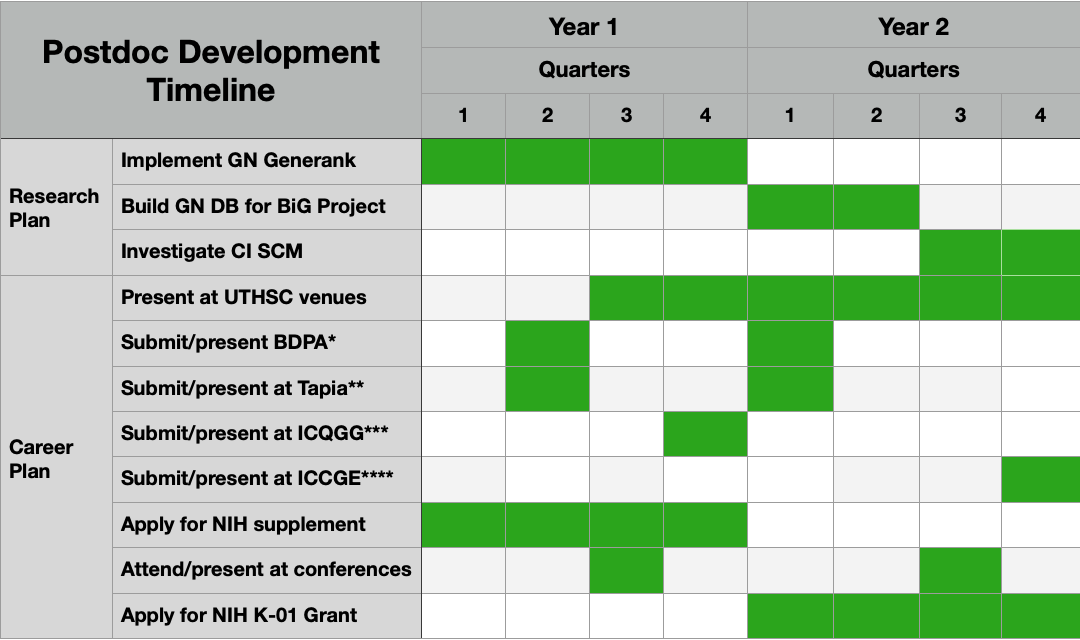
\includegraphics[width=\textwidth]{Figures/timeline-postdoc.eps}
	\caption{\textbf{Postdoc Timeline}\\
	* - Black Data Processing Associates, bdpa.org \\
	** - ACM/CMD-IT Tapia Celebration of Diversity in Computing\\
	*** - International Conference on Quantitative Genetics and Genomics\\
	**** - International Conference on Computational Genomics and Evolution
	}
	\label{fig:timeline}
\end{figure*}


%\includegraphics[width=0.4\textwidth, angle=0]{image1.pdf}